\documentclass[11pt]{article}
\usepackage{geometry}                % See geometry.pdf to learn the layout
\usepackage{graphicx}
\usepackage{amssymb}
\usepackage{epstopdf}

\title{Compte-rendu du TEA "Le compte est bon"}
\author{\textsc{Valentin GAUTHIER}\\ Alexandre TORRES--LEGUET}

\begin{document}
\maketitle

\section{Introduction}
%présentation du problème, le contexte

\quad \quad Ce compte-rendu présente le travail de recherche réalisé pour l’élaboration du code permettant la résolution du jeu "le compte est bon". Après le TP de la séance 2 d’AAP, nous avions à disposition plusieurs fichiers que nous avons  utilisé dans la réalisation du code. Parmi eux, les fichiers :

\begin{itemize}
\item \texttt{list.h} et \texttt{list.c} qui implémentent les listes chaînées.
\item \texttt{stack\textunderscore cs.h} et \texttt{stack\textunderscore cs.c} qui implémentent les piles en contigu statique.
\item \texttt{stack\textunderscore cd.h} et \texttt{stack\textunderscore cd.c} qui implémentent les piles en contigu dynamique.
\item \texttt{stack\textunderscore cld.h} et \texttt{stack\textunderscore cld.c} qui implémentent les piles avec une liste chaînée.
\end{itemize}

Ces fichiers n’ont pas eu à être modifié. 

Nous avons eu a créer ou modifier les fichiers :

\begin{itemize}
\item \texttt{elt.h} et \texttt{elt.c} pour l'implémentation du \texttt{T\textunderscore elt} RPN, qui est une structure possédant 2 champs, dont l'un deux est défini par un ensemble de constantes symboliques également définies dans \texttt{elt.h}. Ils présentent également la fonction toString pour afficher sous forme de string un \texttt{T\textunderscore elt} RPN et genElt pour generer un \texttt{T\textunderscore elt} RPN arbitraire.
\item \texttt{rpn.c} et \texttt{rpn.h} pour l'implémentation des fonctions \texttt{s2list}, \texttt{rpn\textunderscore eval} et \texttt{affiche\textunderscore operations\textunderscore rpn}, fonction qui affiche les opérations effectuées lors de l'évaluation d'une RPN, dans le format demandé dans l'énoncé. 
\item \texttt{stack\textunderscore choix.h} qui permet de décider le type d’implémentation souhaité pour les piles (cs, cd, ou cld)
\item \texttt{rec.h} et \texttt{rec.c} où réside l'algorithme de parcours en profondeur à la volée pour chercher la meilleure RPN.
\item \texttt{main.c} pour gérer le programme (et notamment les paramètres passés correspondant aux cartons tirés et à la cible)
\end{itemize}

\section{Développement}
%organisation du programme
%organisation du groupe (qui a fait quoi)
%difficultés

\quad \quad Dans le déroulé de notre travail, il s’est tout d’abord agit de revoir le cours en profondeur pour s’assurer de maîtriser les nouvelles définitions de types, structures et manières d’implémenter sous \textsc{C} pour plus d’efficacité lors de la réalisation pratique. Cette phase de théorie aura durée l’ensemble du weekend (26 et 27/11). Ensuite, Alexandre s’est chargé de rédigé un premier code en \textsc{Python} pour se faire une première idée de l'algorithme proposé. Puis le lundi 28/11, nous nous sommes réunis pour décider des fichiers et exercices à disposition dans le TP que nous pouvions utiliser (intégralement, en partie ou plus ou moins modifié) pour le TEA. L’après midi du lundi aura suffit pour que nous codions les fonctions nécessaires pour la partie 1 du TEA . Sur cette partie Alexandre s’est chargé des fichiers \texttt{rpn.c} et \texttt{rpn.h}, et Valentin s’est lui occupé de la modification des fichiers \texttt{elt.c} et \texttt{elt.h}.

Puis pour la partie 2, nous nous sommes réunies rapidement mardi pour décider qui ferait quelle partie (implémentation de \texttt{rec.c} ou de \texttt{main.c}) et pour discuter de nos premières idées sur les fonctions. Alexandre est donc partie sur la réalisation de la fonction de recherche en profondeur et Valentin le fichier \texttt{main.c}. Nous avons décider de réaliser ce travail le soir même pour s’assurer d’avoir le temps de corriger les erreurs le lendemain, avant la remise du TEA.

Nous avons rencontré quelques difficultés lors de la manipulation des chaînes de caractères, notamment pour la concaténation (nécessaire lors du parcours en profondeur) ou encore pour convertir des nombres en chaîne de caractère ou vice-versa. Egalement, il a fallu s'accorder sur les conventions prises lors de la Partie 1 (que renvoie \texttt{rpn\textunderscore eval} en cas d'une RPN non valide ? comment le détecter ? etc...) pour effectuer la Partie 2 puisque cette seconde partie se base sur les fonctions développées dans la première.

Un autre point de discussion important a été celui de la représentation des cartons restants. Nous avons au départ penser à utiliser une liste, mais nous nous sommes rendus compte par la suite que avoir accès qu'à l'élément en tête de liste allait rendre inutilement compliqué la boucle à faire sur les cartons restants. Nous avons donc décidé de passer, lors des appels récursifs, un tableau d'entiers ainsi que la longueur de ce tableau.

\section{Résultats}
%présentation des résultats, jeux d'essais, analyse, temps d'exec...

Voici, pour 2 jeux d'essais, les temps d'exécutions constatés sur l'une de nos machines (par moyenne).
Le premier exemple correspond à une cible parfaite, tandis que le second ne peut qu'être approché, d'où la longueur de l'exécution.

\begin{center}
\begin{tabular}{||c c c||} 
 \hline
 cartons & cible & temps \\ [0.5ex] 
 \hline\hline
 3 5 7 9 25 50 & 788 & 1.2s \\ 
 \hline
 2 2 3 4 6 10 & 631 & 23.6s \\ [1ex] 
\hline
\end{tabular}
\end{center}

Il est intéressant de remarquer que ces temps d'exécutions sont bien meilleurs que ceux constatés avec notre implémentation \textsc{Python}.

\section{Schéma d'exploration}

Notre algorithme, étant donné un RPN, cherche à lui ajouter un à un tous les opérateurs, puis un à un les cartons restants.
Une amélioration que nous avons effectué est que, si jamais un RPN peut être évalué sous forme d'une valeur (exemple : $1 \; 2 \; +$ qui peut être évalué à $3$) alors lui ajouter un opérateur le rendra nécessairement invalide. Sur le schéma, on voit que cette amélioration évite l'exploration inutile d'un grand nombre de noeuds de l'arbre.

\begin{center}
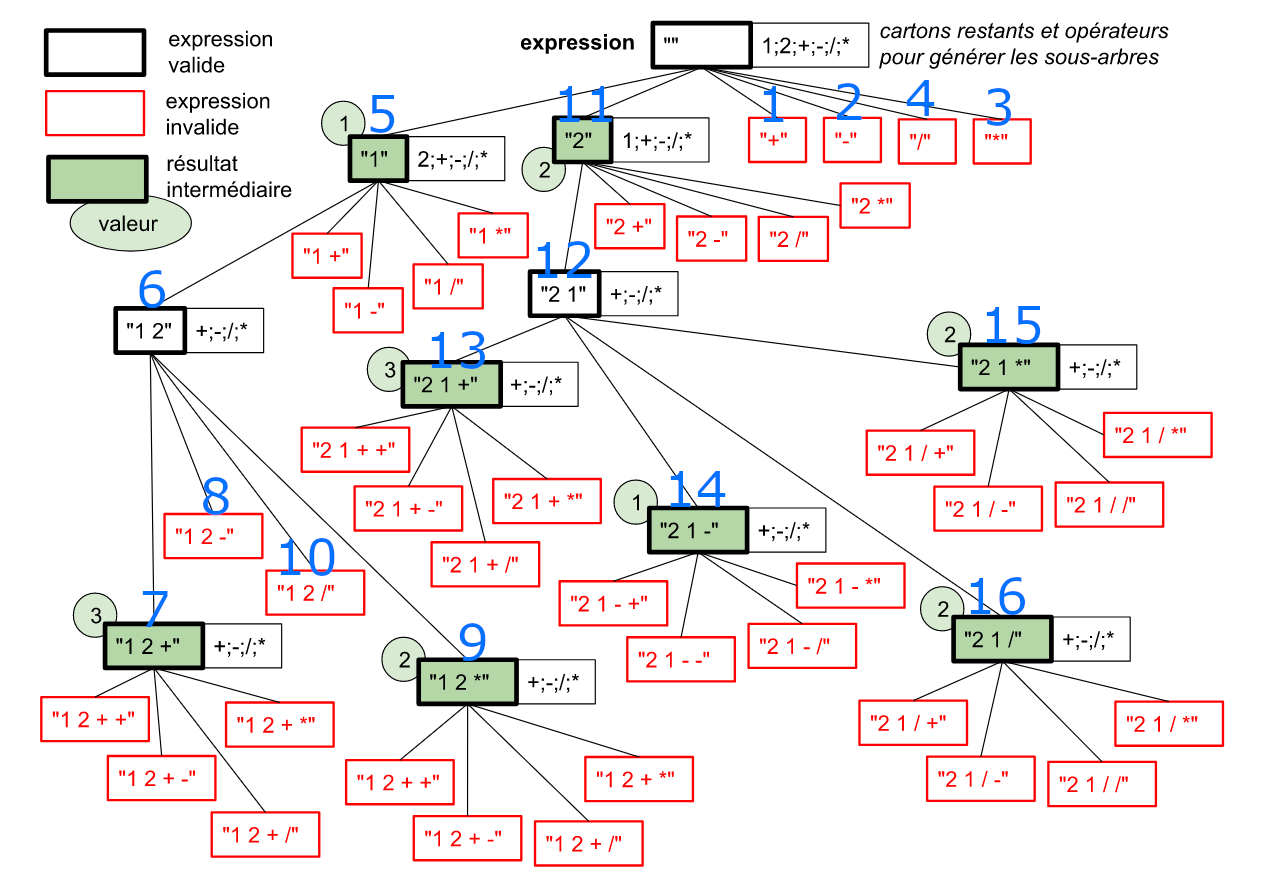
\includegraphics[scale=0.7]{images/arbre_complete.png}
\end{center}

\section{Conclusion}
%analyser les problèmes, perspectives

\quad \quad Au terme du travail, il vient que notre programme semble fonctionner grâce à plusieurs tests tous réalisés avec justesse. Nous restons conscients que c'est un algorithme de type "glouton".



\end{document}  
